% =============================================================================
%  2B. Presentacion en video: avance del proyecto de investigacion
%  Maestria en Ciencia de Datos e Informacion - INFOTEC
%  David Segundo Garcia
%
%  Compilar:  latexmk -pdf presentacion_2b.tex
% =============================================================================
\documentclass[aspectratio=169,11pt]{beamer}

\usepackage[T1]{fontenc}
\usepackage[utf8]{inputenc}
\usepackage[spanish,es-noquoting,es-nolists,es-noshorthands]{babel}
\usepackage{graphicx}
\usepackage{booktabs}
\usepackage{colortbl}   % \rowcolor en la tabla del estado del arte
\usepackage{amsmath,amssymb}
\usepackage{tikz}
\usetikzlibrary{positioning,arrows.meta}

\graphicspath{{figuras/}}

% -----------------------------------------------------------------------------
%  Identidad visual
% -----------------------------------------------------------------------------
\definecolor{vino}{HTML}{7A1B3D}
\definecolor{naranja}{HTML}{E0701E}
\definecolor{grafito}{HTML}{2F3336}
\definecolor{humo}{HTML}{6B7280}
\definecolor{clarito}{HTML}{F4F1EE}

\usetheme{default}
\setbeamertemplate{navigation symbols}{}
\setbeamercolor{structure}{fg=vino}
\setbeamercolor{frametitle}{fg=vino}
\setbeamercolor{title}{fg=vino}
\setbeamercolor{normal text}{fg=grafito}
\setbeamercolor{itemize item}{fg=naranja}
\setbeamercolor{itemize subitem}{fg=humo}
\setbeamertemplate{itemize item}{\raisebox{0.15ex}{\scriptsize$\blacksquare$}}
\setbeamertemplate{itemize subitem}{\raisebox{0.15ex}{\tiny$\bullet$}}
\setbeamerfont{frametitle}{size=\large,series=\bfseries}
\setbeamerfont{title}{size=\LARGE,series=\bfseries}

% titulo con filete inferior
\setbeamertemplate{frametitle}{%
  \vspace{0.55em}%
  \hspace{0.4em}\insertframetitle\par
  \hspace{0.4em}{\color{naranja}\rule{0.30\textwidth}{1.6pt}}\par
  \vspace{-0.2em}%
}

% pie de pagina
\setbeamertemplate{footline}{%
  \hbox{%
    \begin{beamercolorbox}[wd=.80\paperwidth,ht=2.4ex,dp=1.2ex,leftskip=1em]{}%
      {\color{humo}\scriptsize Equidad geográfica en estratificación de riesgo clínico\; ·\;
       David Segundo García}%
    \end{beamercolorbox}%
    \begin{beamercolorbox}[wd=.20\paperwidth,ht=2.4ex,dp=1.2ex,rightskip=1em]{}%
      \hfill{\color{naranja}\scriptsize\bfseries\insertframenumber}%
    \end{beamercolorbox}}%
  \vspace{2pt}%
}

% bloque destacado propio
\newenvironment{clave}[1]
  {\begin{beamercolorbox}[wd=\textwidth,sep=0.6em,rounded=true]{}%
   \setbeamercolor{block}{bg=clarito}%
   \begin{block}{#1}}
  {\end{block}\end{beamercolorbox}}

\newcommand{\resalta}[1]{{\color{vino}\bfseries #1}}
\newcommand{\cifra}[1]{{\color{naranja}\bfseries #1}}

% -----------------------------------------------------------------------------
\title{Estratificación de riesgo clínico consciente de la equidad}
\subtitle{Auditoría y mitigación del sesgo geográfico entre entidades
federativas en modelos predictivos con datos abiertos de salud de México}
\author{David Segundo García}
\institute{Maestría en Ciencia de Datos e Información\\ INFOTEC}
\date{Septiembre de 2026}

\begin{document}

% ============================== 1. PORTADA ===================================
{\setbeamertemplate{footline}{}
\begin{frame}[plain]
  \vspace{0.3em}
  \hfill
\includegraphics[height=0.9cm]{infotec_logo.png}

  \vspace{0.6em}
  {\color{naranja}\rule{\textwidth}{2pt}}

  \vspace{1.0em}
  {\LARGE\bfseries\color{vino} Estratificación de riesgo clínico\\[0.15em]
   consciente de la equidad\par}

  \vspace{0.7em}
  {\small\color{grafito} Auditoría y mitigación del sesgo geográfico entre
  entidades federativas\\ en modelos predictivos con datos abiertos de salud de
  México\par}

  \vspace{1.3em}
  {\color{humo}\rule{0.35\textwidth}{0.6pt}}

  \vspace{0.8em}
  {\normalsize\bfseries David Segundo García\par}
  {\small\color{humo} Proyecto terminal · Maestría en Ciencia de Datos e
  Información\\ Asesor: Dr.\ Daniel Alejandro Cervantes Cabrera\par}

  \vfill
  {\scriptsize\color{humo} Segunda entrega · Septiembre de 2026\par}
\end{frame}}

% ============================== 3. ORIGINALIDAD ==============================
\begin{frame}{Por qué este tema}
  \vspace{0.3em}
  \begin{columns}[T,onlytextwidth]
    \begin{column}{0.52\textwidth}
      \textbf{Lo que ya está hecho}
      \begin{itemize}
        \item Predecir mortalidad por COVID-19 con datos mexicanos ha sido
              \resalta{ampliamente estudiado}.
        \item Los trabajos revisados convergen en niveles de desempeño
              similares.
      \end{itemize}

      \vspace{0.8em}
      \textbf{Lo que no}
      \begin{itemize}
        \item Si ese desempeño es \resalta{el mismo en todo el país}.
        \item En la literatura revisada no se identificaron trabajos que traten
              la \resalta{entidad federativa} como atributo sensible.
      \end{itemize}
    \end{column}
    \begin{column}{0.44\textwidth}
      \vspace{0.6em}
      \setbeamercolor{block body}{bg=clarito}
      \begin{block}{Por qué importa en México}
        La organización federal de los servicios de salud hace que la entidad
        no sea una variable demográfica cualquiera: es la unidad en la que se
        \resalta{decide, se financia y se opera} la atención.

        \vspace{0.5em}
        Un atributo sensible que coincide con la unidad administrativa de
        decisión tiene una propiedad poco común: \resalta{la corrección es
        implementable}.
      \end{block}
    \end{column}
  \end{columns}
\end{frame}

% ============================== 4. CASO DE REFERENCIA ========================
\begin{frame}{El sesgo algorítmico en salud no es hipotético}
  \vspace{0.5em}
  \begin{center}
  \resizebox{\textwidth}{!}{%
  \begin{tikzpicture}[
      node distance=0.7cm,
      caja/.style={draw=humo,rounded corners=2pt,align=center,
                   font=\footnotesize,inner sep=6pt,text width=3.0cm,
                   minimum height=1.5cm},
      flecha/.style={-{Stealth[length=5pt]},draw=naranja,thick}]
    \node[caja,fill=clarito] (a) {Modelo de gestión\\ poblacional\\ \textit{(EE.\,UU.)}};
    \node[caja,fill=clarito,right=of a] (b) {Usa el \textbf{gasto\\ sanitario} como medida\\ de \textbf{necesidad}};
    \node[caja,fill=clarito,right=of b] (c) {Menos acceso\\ $\Rightarrow$ menos gasto\\ con igual enfermedad};
    \node[caja,fill=vino!12,draw=vino,right=of c] (d) {\textbf{Menos recursos}\\ a pacientes\\ afroamericanos};
    \draw[flecha] (a) -- (b);
    \draw[flecha] (b) -- (c);
    \draw[flecha] (c) -- (d);
  \end{tikzpicture}}
  \end{center}

  \vspace{0.4em}
  {\footnotesize\color{humo}\hfill Obermeyer et al.\ (2019), \textit{Science}\hfill}

  \vspace{0.6em}
  \begin{columns}[T,onlytextwidth]
    \begin{column}{0.47\textwidth}
      \setbeamercolor{block body}{bg=clarito}
      \begin{block}{Lección 1}
        El modelo \resalta{no usaba la raza}. Omitir el atributo sensible no
        garantiza equidad.
      \end{block}
    \end{column}
    \begin{column}{0.47\textwidth}
      \setbeamercolor{block body}{bg=clarito}
      \begin{block}{Lección 2}
        El sesgo estaba en la \resalta{definición del desenlace}, no en el
        algoritmo.
      \end{block}
    \end{column}
  \end{columns}
\end{frame}

% ============================== 5. PLANTEAMIENTO =============================
\begin{frame}{Planteamiento del problema}
  \vspace{0.4em}
  \begin{itemize}
    \item Un modelo puede tener \resalta{excelente desempeño promedio} y, al
          mismo tiempo, ser sistemáticamente menos preciso para habitantes de
          entidades con menor infraestructura.
    \item Entrenado con datos dominados por entidades urbanas, puede
          desempeñarse peor \resalta{justo donde el sistema de salud es más
          débil}: amplifica la inequidad en lugar de reducirla.
  \end{itemize}

  \vspace{0.9em}
  \begin{center}
  \begin{minipage}{0.90\textwidth}
    \setbeamercolor{block body}{bg=vino!10}
    \begin{block}{}
      \centering\large
      Medir la inequidad del modelo y corregirla\\
      —especialmente la geográfica—\\
      \resalta{sin sacrificar su utilidad clínica}.
    \end{block}
  \end{minipage}
  \end{center}

  \vspace{0.7em}
  {\footnotesize\color{humo} El objeto de estudio se desplaza: del acierto del
  modelo, a la \textit{distribución} de sus errores entre grupos de
  población.}
\end{frame}

% ============================== 5. PREGUNTAS Y OBJETIVOS =====================
\begin{frame}{Preguntas de investigación y objetivos}
  \vspace{0.3em}
  \begin{columns}[T,onlytextwidth]
    \begin{column}{0.50\textwidth}
      {\bfseries\color{vino} Preguntas}
      \vspace{0.3em}
      {\small
      \begin{itemize}\setlength\itemsep{0.3em}
        \item[\textcolor{naranja}{\bfseries P1}] ¿Hay disparidades entre
              \resalta{entidades}, edades y sexos?
        \item[\textcolor{naranja}{\bfseries P2}] ¿Se asocian al grado de
              \resalta{marginación}?
        \item[\textcolor{naranja}{\bfseries P3}] ¿Qué mitigación funciona, y a
              \resalta{qué costo}?
        \item[\textcolor{naranja}{\bfseries P4}] ¿Se conservan en una
              \resalta{fuente distinta}?
        \item[\textcolor{naranja}{\bfseries P5}] ¿Hay inequidades
              \resalta{interseccionales}?
      \end{itemize}}
    \end{column}
    \begin{column}{0.47\textwidth}
      {\bfseries\color{vino} Objetivo general}
      \vspace{0.3em}

      \setbeamercolor{block body}{bg=clarito}
      \begin{block}{}
        \small Desarrollar un modelo de estratificación de riesgo,
        \resalta{auditar su equidad} —evaluar su desempeño por separado en cada
        grupo— y \resalta{mitigar} las disparidades encontradas.
      \end{block}

      \vspace{0.5em}
      {\footnotesize\color{humo} Cinco objetivos específicos, del flujo
      reproducible con control de fuga de información hasta las recomendaciones
      de despliegue.\par
      \vspace{0.3em}
      Cuatro hipótesis, que se contrastan al final.}
    \end{column}
  \end{columns}
\end{frame}

% ============================== 6. ANTECEDENTES Y ESTADO DEL ARTE ============
\begin{frame}{Antecedentes y estado del arte}
  \vspace{0.2em}
  {\footnotesize Tres tradiciones que avanzaron por separado: la
  \resalta{predicción con datos mexicanos}, la \resalta{epidemiología espacial}
  y la \resalta{equidad algorítmica en salud}. El problema pertenece al ámbito
  donde se cruzan.}

  \vspace{0.6em}
  \centering
  \renewcommand{\arraystretch}{1.20}
  {\footnotesize
  \begin{tabular}{p{4.4cm} p{3.4cm} p{4.6cm}}
    \toprule
    \textbf{Dimensión} & \textbf{En la literatura} & \textbf{Aporte de esta tesis}\\
    \midrule
    Predicción del desenlace (México) & Ampliamente estudiada &
      Línea de base, no aportación\\
    Geografía como predictor (México) & Estudiada &
      Se distingue: geografía como \textit{eje de equidad}\\
    Equidad algorítmica en salud & Madura, fuera de México &
      Se traslada al contexto mexicano\\
    \rowcolor{clarito} Auditoría de equidad por entidad & No identificada en la revisión &
      \textbf{Eje central del trabajo}\\
    \rowcolor{clarito} Mitigación y frontera de Pareto & No identificada en la revisión &
      Instrumento de decisión entregable\\
    \bottomrule
  \end{tabular}}

  \vspace{0.6em}
  {\footnotesize\color{humo} Que la entidad \textit{prediga} la mortalidad no
  dice nada sobre si el modelo es \textit{igualmente confiable} en cada entidad.}
\end{frame}

% ============================== 11. BASES TEORICAS I =========================
\begin{frame}{Bases teóricas: dos propiedades que se confunden}
  \vspace{0.4em}
  \begin{columns}[T,onlytextwidth]
    \begin{column}{0.47\textwidth}
      \setbeamercolor{block body}{bg=clarito}
      \begin{block}{Discriminación}
        \small ¿Ordena bien a los pacientes por riesgo? Se resume en el AUROC.

        \vspace{0.4em}
        Depende \resalta{solo del orden}, no del valor del puntaje.
      \end{block}
      \vspace{0.5em}
      \setbeamercolor{block body}{bg=clarito}
      \begin{block}{Calibración}
        \small De cada cien pacientes con riesgo estimado de 20\,\%,
        ¿fallecen veinte?

        \vspace{0.4em}
        \resalta{La auditoría se hace sobre el puntaje calibrado.}
      \end{block}
    \end{column}
    \begin{column}{0.49\textwidth}
      {\bfseries Criterios formales de equidad}
      \vspace{0.4em}
      {\small
      \begin{itemize}\setlength\itemsep{0.45em}
        \item \resalta{Independencia} — igual tasa de selección entre grupos.
        \item \resalta{Separación} — igual sensibilidad y tasa de falsos
              positivos \\ {\footnotesize(\textit{equalized odds},
              Hardt et al., 2016)}.
        \item \resalta{Suficiencia} — un riesgo de 0.3 significa lo mismo en
              cada entidad.
      \end{itemize}}

      \vspace{0.6em}
      {\footnotesize\color{humo} Sin calibrar, el error por grupo mide el sesgo
      global de entrenamiento y no la inequidad: en este trabajo,
      \cifra{0.2108} frente a \cifra{0.0231}.}
    \end{column}
  \end{columns}
\end{frame}

% ============================== 12. IMPOSIBILIDAD ============================
\begin{frame}{El resultado teórico central: imposibilidad}
  \vspace{0.6em}
  \begin{center}
  \begin{minipage}{0.90\textwidth}
    \setbeamercolor{block body}{bg=vino!10}
    \begin{block}{}
      \centering
      Si la \resalta{prevalencia difiere} entre grupos y el clasificador
      \resalta{no es perfecto},\\ la calibración por grupo y la separación
      \resalta{no pueden cumplirse a la vez}.
      \vspace{0.3em}

      {\footnotesize Chouldechova (2017); Kleinberg et al.\ (2017)}
    \end{block}
  \end{minipage}
  \end{center}

  \vspace{0.9em}
  \begin{columns}[T,onlytextwidth]
    \begin{column}{0.47\textwidth}
      {\bfseries Las dos condiciones se cumplen aquí}
      \begin{itemize}\small
        \item Las tasas de mortalidad por entidad difieren por un factor de
              \cifra{5.6}.
        \item Ningún modelo de riesgo clínico acierta siempre.
      \end{itemize}
    \end{column}
    \begin{column}{0.49\textwidth}
      {\bfseries Consecuencia práctica}
      \begin{itemize}\small
        \item La calibración es propiedad del \resalta{puntaje}; la sensibilidad
              y el FPR, de la \resalta{regla de decisión}.
        \item Un umbral por entidad \resalta{no altera} la calibración y permite
              elegir \textit{cuál} de las dos tasas se iguala.
      \end{itemize}
    \end{column}
  \end{columns}

  \vspace{0.7em}
  {\footnotesize\color{humo} Es un teorema demostrado: se aplica por deducción,
  no depende de los resultados empíricos.}
\end{frame}

% ============================== 13. PARETO ===================================
\begin{frame}{Del teorema al entregable: la frontera de Pareto}
  \vspace{0.5em}
  \begin{columns}[T,onlytextwidth]
    \begin{column}{0.52\textwidth}
      \vspace{0.3em}
      \begin{itemize}\small\setlength\itemsep{0.45em}
        \item Si los criterios no pueden cumplirse a la vez, el resultado
              adecuado \resalta{no es un único modelo «justo»}.
        \item Cada política de despliegue produce un par:
              \textit{disparidad} y \textit{desempeño}.
        \item La frontera reúne las políticas donde ya no se puede mejorar una
              sin empeorar la otra.
        \item Se traza interpolando entre el umbral global y el umbral por
              entidad:
              \[\tau_g(\alpha)=(1-\alpha)\,\tau+\alpha\,\tau_g,\quad
                \alpha\in[0,1]\]
      \end{itemize}
    \end{column}
    \begin{column}{0.45\textwidth}
      \vspace{0.6em}
      \setbeamercolor{block body}{bg=clarito}
      \begin{block}{Por qué importa}
        La elección entre políticas es \resalta{normativa, no técnica}.

        \vspace{0.5em}
        El entregable traslada esa decisión a quien autoriza el despliegue,
        con \resalta{el costo de cada opción medido}, en lugar de esconderla en
        un valor por omisión.
      \end{block}
    \end{column}
  \end{columns}
\end{frame}

% ============================== 14. METODOLOGIA ==============================
\begin{frame}{Marco metodológico: CRISP-DM con una adaptación}
  \vspace{0.7em}
  \begin{center}
  \resizebox{\textwidth}{!}{%
  \begin{tikzpicture}[
      node distance=0.42cm,
      fase/.style={draw=humo,rounded corners=2pt,align=center,
                   font=\scriptsize,inner sep=5pt,text width=1.85cm,
                   fill=clarito,minimum height=1.15cm},
      nueva/.style={fase,fill=vino!15,draw=vino,thick},
      fl/.style={-{Stealth[length=4pt]},draw=naranja,thick}]
    \node[fase] (f1) {Entendimiento\\ del negocio};
    \node[fase,right=of f1] (f2) {Comprensión\\ de los datos};
    \node[fase,right=of f2] (f3) {Preparación\\ de los datos};
    \node[fase,right=of f3] (f4) {Modelado};
    \node[nueva,right=of f4] (f5) {Evaluación\\ \textbf{en dos niveles}};
    \node[fase,right=of f5] (f6) {Implementación};
    \foreach \a/\b in {f1/f2,f2/f3,f3/f4,f4/f5,f5/f6} \draw[fl] (\a) -- (\b);
    \draw[fl,dashed] (f5.south) -- ++(0,-0.5) -| (f4.south);
  \end{tikzpicture}}
  \end{center}

  \vspace{0.8em}
  \begin{columns}[T,onlytextwidth]
    \begin{column}{0.47\textwidth}
      \setbeamercolor{block body}{bg=clarito}
      \begin{block}{La adaptación}
        \small Primero el desempeño \resalta{global}; después el desempeño
        \resalta{desagregado} por grupo. El segundo nivel puede devolver el
        proyecto al modelado \textit{sin que el primero detecte problema
        alguno}.
      \end{block}
    \end{column}
    \begin{column}{0.49\textwidth}
      \setbeamercolor{block body}{bg=clarito}
      \begin{block}{Por qué CRISP-DM}
        \small Cubre el ciclo completo —a diferencia de SEMMA— y es
        independiente de la herramienta. Su límite conocido: no contempla la
        equidad, y por eso se adapta.
      \end{block}
    \end{column}
  \end{columns}
\end{frame}

% ============================== 11. AVANCES ==================================
\begin{frame}{Avances: los datos y el hallazgo principal}
  \vspace{0.2em}
  \begin{columns}[T,onlytextwidth]
    \begin{column}{0.47\textwidth}
      {\footnotesize Base abierta de la DGE, corte 2021, casos confirmados:
      \cifra{2\,526\,649} registros, mortalidad \cifra{5.60\,\%}. Punto de
      predicción: primer contacto. La entidad se \resalta{excluye} como entrada.}

      \vspace{0.5em}
      \setbeamercolor{block body}{bg=vino!10}
      \begin{block}{Aprueba todos los criterios agregados}
        \small AUROC \cifra{0.9503} · sensibilidad \cifra{79.5\,\%} · error de
        calibración \cifra{0.0231}.
      \end{block}

      \vspace{0.4em}
      \centering
      \renewcommand{\arraystretch}{1.12}
      {\footnotesize
      \begin{tabular}{l c}
        \toprule
        \textbf{Eje auditado} & \textbf{Brecha de sensibilidad}\\
        \midrule
        Entidad federativa (32) & \cifra{0.2935}\\
        Sexo (2)                & 0.0393\\
        Grupo etario (4)        & \cifra{0.5824}\\
        \bottomrule
      \end{tabular}}

      \vspace{0.4em}
      {\footnotesize IC \cifra{[0.267,\ 0.354]} · permutación \cifra{$p=0.001$}}
    \end{column}
    \begin{column}{0.50\textwidth}
      \centering
      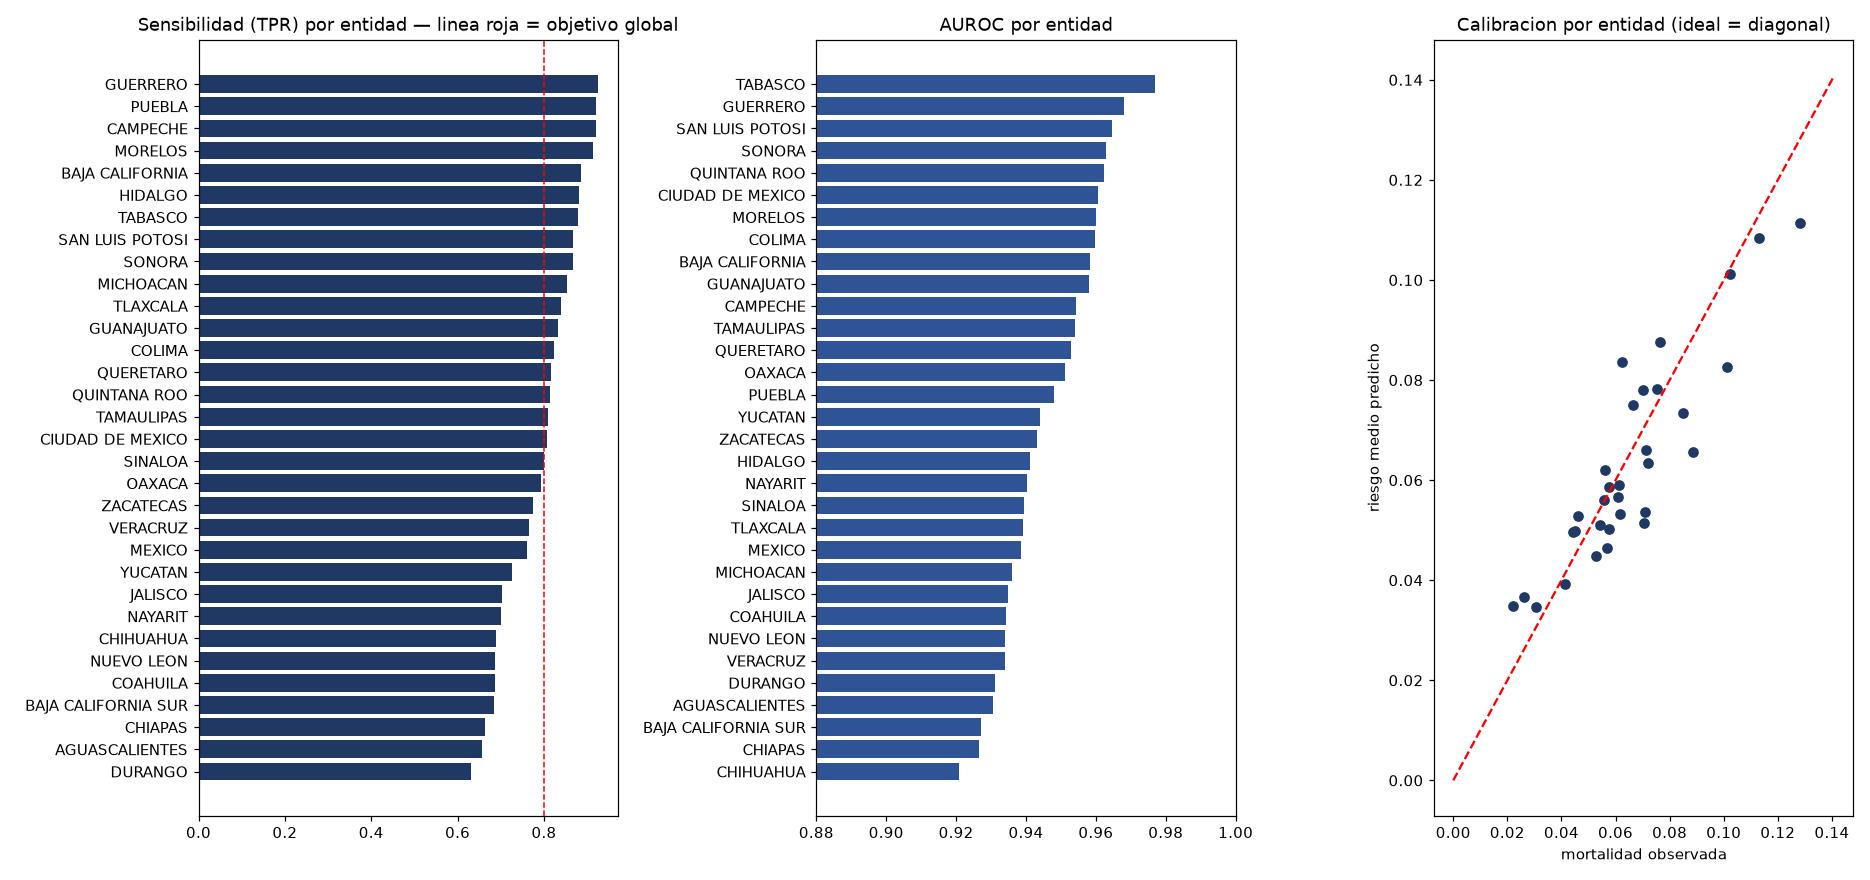
\includegraphics[width=\textwidth]{equidad_por_entidad.png}

      \vspace{0.2em}
      {\scriptsize\color{humo} Desempeño desagregado por entidad federativa.}
    \end{column}
  \end{columns}
\end{frame}

% ============================== 12. HIPOTESIS Y PENDIENTES ===================
\begin{frame}{Las hipótesis y lo que queda pendiente}
  \vspace{0.2em}
  \centering
  \renewcommand{\arraystretch}{1.10}
  {\scriptsize
  \begin{tabular}{p{0.9cm} p{7.4cm} p{3.9cm}}
    \toprule
    & \textbf{Enunciado} & \textbf{Resultado}\\
    \midrule
    \textcolor{naranja}{\bfseries H1} & Un modelo con buen desempeño global
      presentará disparidades entre entidades & \resalta{Sostenida}
      (29.4 puntos)\\
    \textcolor{naranja}{\bfseries H2} & La disparidad se asociará a la
      marginación de la entidad & \resalta{No sostenida}
      ($r=-0.178$, $p=0.328$)\\
    \textcolor{naranja}{\bfseries H3} & La mitigación reducirá la brecha con
      pérdida acotada & \resalta{Sostenida} (0.294 $\to$ 0.140, sin costo)\\
    \textcolor{naranja}{\bfseries H4} & El desempeño se transferirá a una fuente
      independiente & \resalta{Pendiente} de validación externa\\
    \bottomrule
  \end{tabular}}

  \vspace{0.7em}
  \begin{center}
  \begin{minipage}{0.92\textwidth}
    \setbeamercolor{block body}{bg=clarito}
    \begin{block}{La limitación que condiciona todo lo demás}
      \centering\footnotesize
      Restringido a pacientes hospitalizados, el AUROC cae de \cifra{0.9503} a
      \cifra{0.7001}: parte del desempeño aparente consistía en separar
      ambulatorios de hospitalizados.
    \end{block}
  \end{minipage}
  \end{center}
\end{frame}

% ============================== 19. CIERRE ===================================
{\setbeamertemplate{footline}{}
\begin{frame}[plain]
  \vspace{1.6em}
  \centering
  {\color{naranja}\rule{0.45\textwidth}{2pt}}

  \vspace{1.4em}
  {\LARGE\bfseries\color{vino} Gracias\par}

  \vspace{1.2em}
  \begin{minipage}{0.80\textwidth}
    \centering\small\color{grafito}
    Un modelo puede acertar en promedio y fallar de forma sistemática en una
    parte del país.\\[0.35em]
    Medirlo antes de desplegarlo es una decisión de método, no de oportunidad.
  \end{minipage}

  \vspace{1.6em}
  {\small\bfseries David Segundo García\par}
  {\footnotesize\color{humo} Maestría en Ciencia de Datos e Información ·
  INFOTEC\\ Asesor: Dr.\ Daniel Alejandro Cervantes Cabrera\par}

  \vspace{1.0em}
  
\includegraphics[height=0.75cm]{infotec_logo.png}
\end{frame}}

\end{document}
